% Compile this file for printable slides (disable animations and don't waste ink)

\documentclass[handout, xcolor={dvipsnames}]{beamer}\usepackage{etoolbox}\newtoggle{printable}\toggletrue{printable}

% Adjust these for the path of the theme and its graphics, relative to this file
%\usepackage{beamerthemeFalmouthGamesAcademy}
\usepackage{../../beamerthemeFalmouthGamesAcademy}
\usepackage{multimedia}
\graphicspath{ {../../} }

% Default language for code listings
\lstset{language=C++,
        morekeywords={each,in,nullptr}
}

% For strikethrough effect
\usepackage[normalem]{ulem}
\usepackage{wasysym}

\usepackage{pdfpages}

% http://www.texample.net/tikz/examples/state-machine/
\usetikzlibrary{arrows,automata}

\newcommand{\modulecode}{COMP260}\newcommand{\moduletitle}{Distributed Systems}\newcommand{\sessionnumber}{5}

\setbeamertemplate{navigation symbols}{}

\newcommand{\fullbleed}[1]{
\begin{frame}[plain]
	\begin{tikzpicture}[remember picture, overlay]
		\node[at=(current page.center)] {
			\includegraphics[width=\paperwidth]{#1}
		};
	\end{tikzpicture}
\end{frame}
}

\newcommand{\picturepage}[2]{
\begin{frame}[plain]
	\begin{tikzpicture}[remember picture, overlay]
		\node[at=(current page.center)] {
			\includegraphics[width=\paperwidth]{#1}
		};
		\draw<1>[draw=none, fill=black, opacity=0.9] (-1,-5.2) rectangle (current page.south east);
		\node[draw=none,text width=0.96\paperwidth, align=right] at (5.5,-5.5) {\tiny{#2}};
	\end{tikzpicture}
\end{frame}
}

\newcommand{\notepicx}[5]{
\begin{frame}[plain]
	\begin{tikzpicture}[remember picture, overlay]
		\node[at=(current page.center)] {
			\includegraphics[width=\paperwidth]{#1}
		};
		\node[draw=none, fill=black, text width=#5\paperwidth] at ([xshift=#3, yshift=#4] current page.center) {\small{#2}};
	\end{tikzpicture}
\end{frame}
}

\newcommand{\notepic}[4]{
	\notepicx{#1}{#2}{#3}{#4}{0.4}
}

\newcommand{\socrative}{
	\begin{center}
		Socrative room code: \texttt{FALCOMPMIKE}
	\end{center}
}

\begin{document}
\title{\sessionnumber: From Concepts to Design}
\subtitle{\modulecode: \moduletitle}

\frame{\titlepage} 

% Adjust these for the path of the theme and its graphics, relative to this file
%\usepackage{beamerthemeFalmouthGamesAcademy}
\usepackage{../../beamerthemeFalmouthGamesAcademy}
\usepackage{multimedia}
\graphicspath{ {../../} }

\usepackage[T1]{fontenc}

% Fixes font encoding issue where £ sign comes out as $ in math mode
\renewcommand{\pounds}{\text{\textsterling}}

% Default language for code listings
\lstset{language=C++,
        morekeywords={each,in,nullptr}
}

% For strikethrough effect
\usepackage[normalem]{ulem}
\usepackage{wasysym}

\usepackage[noend]{algpseudocode}
\usepackage{pdfpages}

% http://www.texample.net/tikz/examples/state-machine/
\usetikzlibrary{arrows,automata}

\newcommand{\modulecode}{COMP260}\newcommand{\moduletitle}{Distributed Systems}\newcommand{\sessionnumber}{5}

\begin{document}
\title{\sessionnumber: Monte Carlo Tree Search}
\subtitle{\modulecode: \moduletitle}

\frame{\titlepage} 

\part{Assignments}
\frame{\partpage}

\begin{frame}{COMP250 assignments}
	\pause Similar to COMP220:
	\begin{itemize}
		\pause\item Portfolio task (90\%)
		\pause\item Research journal (10\%)
	\end{itemize}
\end{frame}

\begin{frame}{COMP250 portfolio task}
	\begin{itemize}
		\pause\item Assignment brief on LearningSpace
		\pause\item Basically, develop an \textbf{AI component} for a game
		\pause\item In the next two weeks:
			\begin{itemize}
				\pause\item Prepare a \textbf{proposal}
				\pause\item Start \textbf{collecting} and \textbf{reading} appropriate literature
			\end{itemize}
		\pause\item For the rest of today: begin preparing your \textbf{proposal}
		\pause\item Not sure what's technically feasible? \textbf{Ask me!}
	\end{itemize}
\end{frame}


% !TeX root = ./2019-20-COMP250-05-session-materials_screen.tex
\part{Monte Carlo evaluation}
\frame{\partpage}

\begin{frame}{Recap}
	\begin{itemize}
		\pause\item It is useful to have a \textbf{heuristic evaluation function} for nonterminal states
		\pause\item Allows 1-ply search, depth-limited minimax, \dots
		\pause\item Designing a good heuristic requires in-depth knowledge of the game
		\pause\item What if you don't have such knowledge?
	\end{itemize}
\end{frame}

\begin{frame}{Monte Carlo methods}
	\begin{itemize}
		\pause\item In computing, a \textbf{Monte Carlo method} is an algorithm based on \textbf{averaging over random samples}
		\pause\item The \textbf{average} over a large number of samples is a good approximation of the \textbf{expected value}
		\pause\item Used for \textbf{quickly approximating} quantities over \textbf{large domains}
		\pause\item Generally designed to \textbf{converge in the limit}
			\begin{itemize}
				\pause\item An \textbf{infinite} number of samples would give an \textbf{exact} answer
				\pause\item As the \textbf{number of samples} increases, the \textbf{accuracy} of the answer improves
			\end{itemize}
		\pause\item Applications in physics, engineering, finance, weather forecasting, graphics, ...
	\end{itemize}
\end{frame}

\begin{frame}{Aside: ``randomness'' in computing}
	\begin{itemize}
		\pause\item Digital computers are \textbf{deterministic}, so there's no such thing as true randomness
			\begin{itemize}
				\pause\item Cryptographically secure systems use an external source of randomness e.g.\ atmospheric noise, radioactive decay
			\end{itemize}
		\pause\item What we actually have are \textbf{pseudo-random number generators (PRNGs)}
		\pause\item A PRNG is an algorithm which gives an \textbf{unpredictable} sequence of numbers based on a \textbf{seed}
		\pause\item Sequence is \textbf{uniformly distributed}, i.e.\ all numbers have equal probability
		\pause\item Seed is generally based on some source of \textbf{entropy}, e.g.\ system clock, mouse input, electronic noise
	\end{itemize}
\end{frame}

\begin{frame}{Monte Carlo evaluation in games}
	\begin{itemize}
		\pause\item Based on \textbf{random rollouts}
	\end{itemize}
	\pause
	\begin{algorithmic}
		\While{$s$ is not terminal}
			\State let $m$ be a random legal move from $s$
			\State update $s$ by playing $m$
		\EndWhile
	\end{algorithmic}
	\begin{itemize}
		\pause\item The \textbf{value} of a rollout is the \textbf{value} of the terminal state it reaches (i.e.\ $1$ for a win, $-1$ for a loss, $0$ for a draw)
		\pause\item Averaging gives the \textbf{expected value} of the initial state
		\pause\item Higher expected value $=$ more chance of winning
	\end{itemize}
\end{frame}

\begin{frame}{Monte Carlo search}
	\begin{itemize}
		\pause\item \textbf{Flat Monte Carlo search}: 1-ply search with Monte Carlo evaluation
		\pause\item How about minimax with $d>1$ and Monte Carlo evaluation?
			\begin{itemize}
				\pause\item Minimax assumes the evaluation is \textbf{deterministic}, but Monte Carlo is not
				\pause\item Not commonly used, mainly because there's something better...
			\end{itemize}
	\end{itemize}
\end{frame}


% !TeX root = ./2020-21-COMP250-05-session-materials_screen.tex
\part{Monte Carlo Tree Search}
\frame{\partpage}

\begin{frame}{Monte Carlo Tree Search (MCTS)}
	\begin{itemize}
		\pause\item Like Monte Carlo evaluation, based on \textbf{rollouts}
		\pause\item First few rollouts are \textbf{random}
		\pause\item However, statistics from these rollouts are used to \textbf{bias} future rollouts
		\pause\item Bias rollouts towards \textbf{plausible} lines of play,
			i.e.\ where each player is trying to play the best move
	\end{itemize}
\end{frame}

\begin{frame}{The MCTS algorithm}
	\begin{itemize}
		\pause\item MCTS builds a \textbf{subtree} of the game tree
		\pause\item Initially, the tree consists of a single \textbf{root node}
		\pause\item Each rollout has four stages:
			\begin{itemize}
				\pause\item \textbf{Selection}: Starting from the root, descend the tree by choosing moves.
					Continue until we reach a node which does not yet have children for all legal moves.
				\pause\item \textbf{Expansion}: Choose a random legal move for which the current node does not have a child node.
					Add this new node to the tree.
				\pause\item \textbf{Simulation}: Perform a Monte Carlo rollout, playing random moves until a terminal state is reached.
				\pause\item \textbf{Backpropagation}: For each node visited during \textbf{selection} and \textbf{expansion},
					update the node's statistics based on the result of the simulation.
			\end{itemize}
		\pause\item Perform many rollouts, then use the statistics at the top level of the tree to choose the best move
	\end{itemize}
\end{frame}

\begin{frame}{The MCTS algorithm}
	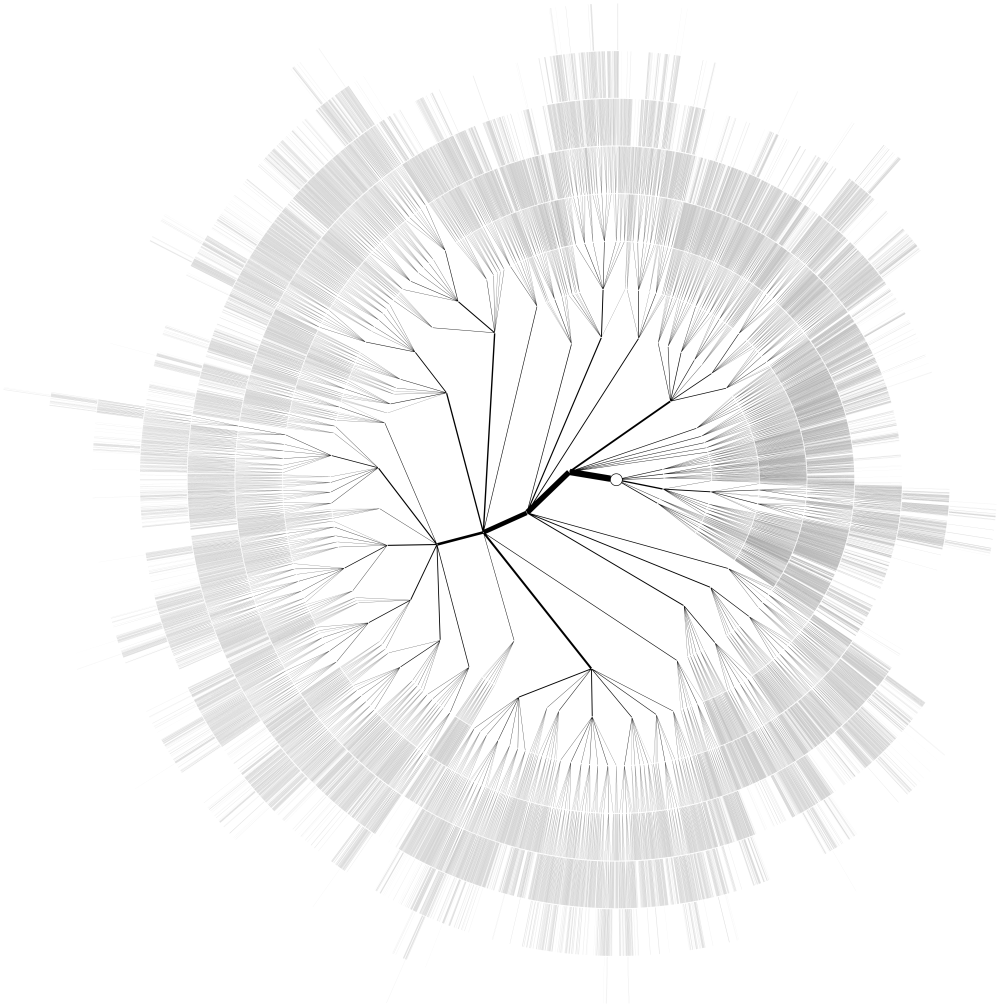
\includegraphics[width=\textwidth]{mcts}
\end{frame}

\begin{frame}{Selection policy}
	\begin{itemize}
		\pause\item Selection must balance:
			\begin{itemize}
				\pause\item \textbf{Exploitation} of moves that are known to be good
				\pause\item \textbf{Exploration} of moves that have not often been tried
			\end{itemize}
		\pause\item This can be modelled as a \textbf{multi-armed bandit problem}
	\end{itemize}
\end{frame}

\begin{frame}{Multi-armed bandits}
	\begin{itemize}
		\pause\item We have a row of one-armed bandits (slot machines)
		\pause\item We \textbf{do not know} the payout probabilities of any of them, and they're all different
		\pause\item How to maximise our winnings?
		\pause\item Again must balance
			\begin{itemize}
				\pause\item \textbf{Exploitation} of machines that are known to have a high expected payout
				\pause\item \textbf{Exploration} of machines that have not been tried often, to get a better estimate of their expected payout
			\end{itemize}
	\end{itemize}
\end{frame}

\begin{frame}{Upper Confidence Bound (UCB)}
	\begin{itemize}
		\pause\item For each machine $m$, record:
			\begin{itemize}
				\pause\item $n_m$: the number of plays of this machine
				\pause\item $V_m$: the total winnings from playing this machine
				\pause\item $n = \sum_m n_m$, total number of plays across all machines
			\end{itemize}
		\pause\item At each stage, play the machine for which
			$$ \frac{V_m}{n_m} + c \sqrt{ \frac{\log n}{n_m} } $$
			is largest
			\begin{itemize}
				\pause\item $\frac{V_m}{n_m}$ is the \textbf{exploitation} part: average payout from this machine so far
				\pause\item $\sqrt{ \frac{\log n}{n_m} }$ is the \textbf{exploration} part: large if $n_m$ is small
				\pause\item $c$ is a parameter for adjusting the balance between exploitation and exploration
			\end{itemize}
	\end{itemize}
\end{frame}

\begin{frame}{UCB demo}
	\begin{center}
		\url{http://orangehelicopter.com/academic/bandits.html?ucb}
	\end{center}
\end{frame}

\begin{frame}{Upper Confidence Bound for Trees (UCT)}
	\begin{itemize}
		\pause\item Use UCB as the selection policy
		\pause\item In each node $x$, record:
			\begin{itemize}
				\pause\item $n_x$: the number of visits to this node
				\pause\item $V_x$: the total value of rollouts through this node
			\end{itemize}
		\pause\item From node $p$, choose the child $q$ such that
			$$ \frac{V_q}{n_q} + c \sqrt{ \frac{\log n_p}{n_q} } $$
			is largest
	\end{itemize}
\end{frame}

\begin{frame}{UCT demo}
	\begin{center}
		\texttt{InteractiveDemo.exe}
	\end{center}
\end{frame}

\begin{frame}{Benefits of MCTS}
	\begin{itemize}
		\pause\item ``Vanilla'' MCTS is \textbf{game independent}
		\pause\item But if game-specific heuristics are available, they can be used to \textbf{enhance} MCTS
		\pause\item MCTS is \textbf{anytime}
			\begin{itemize}
				\pause\item Can stop it after \textbf{any} amount of computation (within reason) and get a reasonably good answer
				\pause\item Compare with minimax: $O(e^d)$ for depth $d$
			\end{itemize}
		\pause\item Does not suffer from \textbf{horizon effect}
			\begin{itemize}
				\pause\item Minimax at depth $d$ cannot ``see'' what happens $d+1$ moves in the future
				\pause\item MCTS can build the tree as deep as it likes
				\pause\item Selects which parts of the tree to expand more deeply
			\end{itemize}
	\end{itemize}
\end{frame}



\end{document}


\end{document}
